\chapter{Missão Típica}
\label{missao_tipica_parte2}
\section{Pista de decolagem}

Tendo em vista que a aeronave projetada operará regionalmente, foi estabelecido que ela deverá ser capaz de decolar e pousar em aeroportos movimentados de comprimento de pista reduzidos.
Desse modo, haverá mais opções de rotas que ela poderá realizar em uma dada região, tornando-a então mais versátil.

Definiu-se portanto que a aeronave deverá ser certificada para certas pistas específicas, listadas abaixo.
Ainda, definiu-se que o motor a ser usado deve ser do tipo turboélice.
Pela figura \ref{fig:motoresVelocidade} percebe-se a maior eficácia dos motores turboélice em comparação com outros motores a reação, o que justifica sua escolha para o projeto.

\begin{figure}[H]
  \label{fig:motoresVelocidade}
  \caption{Comparação de tração de diferentes tipos de motores em função da velocidade.}
  \centering
    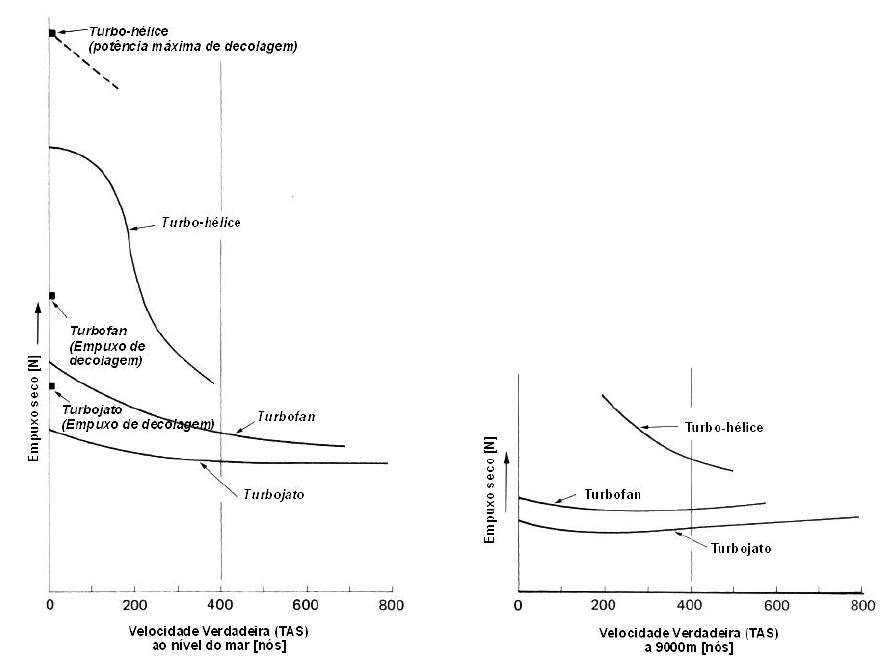
\includegraphics[width=0.95\textwidth]{images/parte2/graficosMotores}
\end{figure}

\subsection{Aeroporto London City (LCY)}

O Aeroporto London City, na cidade de Londres (Inglaterra), situa-se em meio a obstáculos que impõem restrições aos ângulos de decolagem e pouso.
Estes ângulos serão usados para determinar a mínima razão de subida necessária para a aeronave.
As cartas de aproximação e decolagem do aeroporto estão na página \pageref{anexoB}.

\subsection{Aeroporto Santos Dumont (SDU)}

O Aeroporto Santos Dumont, no Rio de Janeiro, se localiza em uma parte central da cidade, o que justifica sua grande movimentação.
A menor de suas duas pistas -- a auxiliar -- conta com 1260 metros de comprimento por 30 metros de largura \cite{AISWEB:aerodromos}.
As cartas de aproximação e decolagem do aeroporto estão na página \pageref{anexoB}.
